\section{Freestart collisions for 80-step SHA-1}
\label{sec:res_80}

This section gives the attack parameters for the 80-step (full) freestart collision attack on \shaone.

\subsection{The differential path for part of the two first rounds}
\label{sec:app_diff_path80}

A graphical representation of the differential path
used in our attack up to step 28 is given in \autoref{fig:diff_path80}.
It consists of sufficient conditions for the state, and of the associated message signed bit differences.
The meaning of the bit condition symbols were defined in \autoref{table:appbitconditions}.
Note that the signs of message bit differences are enforced through message bit relations.
The message bit relations
used in the attack past $\expmess_{28}$ are given in \autoref{fig:msgbitrel80}, and a graphical
representation thereof in
\autoref{fig:msgbitrel80_graph}.
The remainder of the path can easily be determined by linearisation of the step function given the differences
in the message.

\begingroup
\fontsize{8pt}{9pt}\selectfont
\begin{verbbox}
A-4: ........ ........ ........ ........
A-3: ........ ........ ........ ........
A-2: ........ ........ ........ .....^-.
A-1: 1...1... ........ ........ .0.....+
A0 : 01..0... ........ ........ .1......  W0 : x.+...+. ........ ........ ...+....
A1 : 11+^..+. ........ ....^... ...+....  W1 : ..-..-.. ........ ........ ...-++..
A2 : ..-11-1. 1......^ .....1+1 10.1.0..  W2 : ..+..--. ........ ........ ...-.+..
A3 : .0.0-001 1.^.10.. .+01.011 11^0.1.1  W3 : ..-..--. ........ ........ ...-+.-.
A4 : .1.11+-1 +^^^+1^^ ^011^^.- +++++-.+  W4 : ........ ........ ........ ...+....
A5 : .+.+.-++ ++++++++ ++++++++ .+0-1111  W5 : .....-.. ........ ........ ...+++..
A6 : .0.0.1.0 11.111.1 1110-010 0-1.10-+  W6 : x+..++.. ........ ........ ...-.+..
A7 : 1-.+.1.0 10100010 00000011 1+.-.0.+  W7 : ....-+.. ........ ........ ......+.
A8 : 0+.0.0.. ........ ......0. .+.-.0.1  W8 : x-...... ........ ........ ...+....
A9 : .+.0.0.. ........ ........ .0.+...^  W9 : x.-+.-.. ........ ........ ...-++..
A10: .+...... ........ ........ ...+.0..  W10: ..-+++.. ........ ........ .....-..
A11: ...-.... ........ ........ ........  W11: x.++++.. ........ ........ ...-+.+.
A12: ...0.1.. ........ ........ .....1..  W12: ..-..... ........ ........ ...-....
A13: .1...0.. ........ ........ ......!^  W13: ..+..+.. ........ ........ ...-++..
A14: +-...... ........ ........ ........  W14: x++.+-.. ........ ........ ...-.+..
A15: 1.1-.... ........ ........ ......!.  W15: ....+-.. ........ ........ ......+.
A16: +.10.1.. ........ ........ ........  W16: x+...... ........ ........ ...-....
A17: 1.-..0.. ........ ........ .......^  W17: x.++.+.. ........ ........ ...+--..
A18: .+-.0... ........ ........ .......!  W18: ..+.--.. ........ ........ .....-..
A19: .+.s.... ........ ........ ........  W19: x.+---.. ........ ........ ...-+...
A20: -...R... ........ ........ ........  W20: x.++.... ........ ........ ...+....
A21: -.+R.... ........ ........ ........  W21: ........ ........ ........ ....++..
A22: -...S... ........ ........ .......^  W22: x.---... ........ ........ ...+....
A23: .-..R... ........ ........ ........  W23: ....-... ........ ........ ...+-...
A24: -.rs.... ........ ........ ........  W24: .-+--... ........ ........ ...+....
A25: -.-r.... ........ ........ ........  W25: ....+... ........ ........ ...+.+..
A26: -...s... ........ ........ ........  W26: .+--.... ........ ........ ...+....
A27: -.-.r... ........ ........ ........  W27: x.+-+... ........ ........ ...++-..
A28: ........ ........ ........ ........  W28: x+-.-... ........ ........ ........
A29: ..-..... ........ ........ ........
\end{verbbox}
\endgroup

\begin{figure}[!htb]
\centering
\begin{tabular}{lcc}
$i$ & $\state_i$ & $\mess_i$\\
-4 & \nodiff\nodiff\nodiff\nodiff\nodiff\nodiff\nodiff\nodiff\nodiff\nodiff\nodiff\nodiff\nodiff\nodiff\nodiff\nodiff\nodiff\nodiff\nodiff\nodiff\nodiff\nodiff\nodiff\nodiff\nodiff\nodiff\nodiff\nodiff\nodiff\nodiff\nodiff\nodiff \\
-3 & \nodiff\nodiff\nodiff\nodiff\nodiff\nodiff\nodiff\nodiff\nodiff\nodiff\nodiff\nodiff\nodiff\nodiff\nodiff\nodiff\nodiff\nodiff\nodiff\nodiff\nodiff\nodiff\nodiff\nodiff\nodiff\nodiff\nodiff\nodiff\nodiff\nodiff\nodiff\nodiff \\
-2 & \nodiff\nodiff\nodiff\nodiff\nodiff\nodiff\nodiff\nodiff\nodiff\nodiff\nodiff\nodiff\nodiff\nodiff\nodiff\nodiff\nodiff\nodiff\nodiff\nodiff\nodiff\nodiff\nodiff\nodiff\nodiff\nodiff\nodiff\nodiff\nodiff\equaup$\monediffd$\nodiff \\
-1 & $\mnodiffo$\nodiff\nodiff\nodiff$\mnodiffo$\nodiff\nodiff\nodiff\nodiff\nodiff\nodiff\nodiff\nodiff\nodiff\nodiff\nodiff\nodiff\nodiff\nodiff\nodiff\nodiff\nodiff\nodiff\nodiff\nodiff$\mnodiffz$\nodiff\nodiff\nodiff\nodiff\nodiff$\monediffu$ \\
0  & $\mnodiffz$$\mnodiffo$\nodiff\nodiff$\mnodiffz$\nodiff\nodiff\nodiff\nodiff\nodiff\nodiff\nodiff\nodiff\nodiff\nodiff\nodiff\nodiff\nodiff\nodiff\nodiff\nodiff\nodiff\nodiff\nodiff\nodiff$\mnodiffo$\nodiff\nodiff\nodiff\nodiff\nodiff\nodiff  &  \onediff\nodiff$\monediffu$\nodiff\nodiff\nodiff$\monediffu$\nodiff\nodiff\nodiff\nodiff\nodiff\nodiff\nodiff\nodiff\nodiff\nodiff\nodiff\nodiff\nodiff\nodiff\nodiff\nodiff\nodiff\nodiff\nodiff\nodiff$\monediffu$\nodiff\nodiff\nodiff\nodiff \\
1  & $\mnodiffo$$\mnodiffo$$\monediffu$\equaup\nodiff\nodiff$\monediffu$\nodiff\nodiff\nodiff\nodiff\nodiff\nodiff\nodiff\nodiff\nodiff\nodiff\nodiff\nodiff\nodiff\equaup\nodiff\nodiff\nodiff\nodiff\nodiff\nodiff$\monediffu$\nodiff\nodiff\nodiff\nodiff  &  \nodiff\nodiff$\monediffd$\nodiff\nodiff$\monediffd$\nodiff\nodiff\nodiff\nodiff\nodiff\nodiff\nodiff\nodiff\nodiff\nodiff\nodiff\nodiff\nodiff\nodiff\nodiff\nodiff\nodiff\nodiff\nodiff\nodiff\nodiff$\monediffd$$\monediffu$$\monediffu$\nodiff\nodiff \\
2  & \nodiff\nodiff$\monediffd$$\mnodiffo$$\mnodiffo$$\monediffd$$\mnodiffo$\nodiff$\mnodiffo$\nodiff\nodiff\nodiff\nodiff\nodiff\nodiff\equaup\nodiff\nodiff\nodiff\nodiff\nodiff$\mnodiffo$$\monediffu$$\mnodiffo$$\mnodiffo$$\mnodiffz$\nodiff$\mnodiffo$\nodiff$\mnodiffz$\nodiff\nodiff  &  \nodiff\nodiff$\monediffu$\nodiff\nodiff$\monediffd$$\monediffd$\nodiff\nodiff\nodiff\nodiff\nodiff\nodiff\nodiff\nodiff\nodiff\nodiff\nodiff\nodiff\nodiff\nodiff\nodiff\nodiff\nodiff\nodiff\nodiff\nodiff$\monediffd$\nodiff$\monediffu$\nodiff\nodiff \\
3  & \nodiff$\mnodiffz$\nodiff$\mnodiffz$$\monediffd$$\mnodiffz$$\mnodiffz$$\mnodiffo$$\mnodiffo$\nodiff\equaup\nodiff$\mnodiffo$$\mnodiffz$\nodiff\nodiff\nodiff$\monediffu$$\mnodiffz$$\mnodiffo$\nodiff$\mnodiffz$$\mnodiffo$$\mnodiffo$$\mnodiffo$$\mnodiffo$\equaup$\mnodiffz$\nodiff$\mnodiffo$\nodiff$\mnodiffo$  &  \nodiff\nodiff$\monediffd$\nodiff\nodiff$\monediffd$$\monediffd$\nodiff\nodiff\nodiff\nodiff\nodiff\nodiff\nodiff\nodiff\nodiff\nodiff\nodiff\nodiff\nodiff\nodiff\nodiff\nodiff\nodiff\nodiff\nodiff\nodiff$\monediffd$$\monediffu$\nodiff$\monediffd$\nodiff \\
4  & \nodiff$\mnodiffo$\nodiff$\mnodiffo$$\mnodiffo$$\monediffu$$\monediffd$$\mnodiffo$$\monediffu$\equaup\equaup\equaup$\monediffu$$\mnodiffo$\equaup\equaup\equaup$\mnodiffz$$\mnodiffo$$\mnodiffo$\equaup\equaup\nodiff$\monediffd$$\monediffu$$\monediffu$$\monediffu$$\monediffu$$\monediffu$$\monediffd$\nodiff$\monediffu$  &  \nodiff\nodiff\nodiff\nodiff\nodiff\nodiff\nodiff\nodiff\nodiff\nodiff\nodiff\nodiff\nodiff\nodiff\nodiff\nodiff\nodiff\nodiff\nodiff\nodiff\nodiff\nodiff\nodiff\nodiff\nodiff\nodiff\nodiff$\monediffu$\nodiff\nodiff\nodiff\nodiff \\
5  & \nodiff$\monediffu$\nodiff$\monediffu$\nodiff$\monediffd$$\monediffu$$\monediffu$$\monediffu$$\monediffu$$\monediffu$$\monediffu$$\monediffu$$\monediffu$$\monediffu$$\monediffu$$\monediffu$$\monediffu$$\monediffu$$\monediffu$$\monediffu$$\monediffu$$\monediffu$$\monediffu$\nodiff$\monediffu$$\mnodiffz$$\monediffd$$\mnodiffo$$\mnodiffo$$\mnodiffo$$\mnodiffo$  &  \nodiff\nodiff\nodiff\nodiff\nodiff$\monediffd$\nodiff\nodiff\nodiff\nodiff\nodiff\nodiff\nodiff\nodiff\nodiff\nodiff\nodiff\nodiff\nodiff\nodiff\nodiff\nodiff\nodiff\nodiff\nodiff\nodiff\nodiff$\monediffu$$\monediffu$$\monediffu$\nodiff\nodiff \\
6  & \nodiff$\mnodiffz$\nodiff$\mnodiffz$\nodiff$\mnodiffo$\nodiff$\mnodiffz$$\mnodiffo$$\mnodiffo$\nodiff$\mnodiffo$$\mnodiffo$$\mnodiffo$\nodiff$\mnodiffo$$\mnodiffo$$\mnodiffo$$\mnodiffo$$\mnodiffz$$\monediffd$$\mnodiffz$$\mnodiffo$$\mnodiffz$$\mnodiffz$$\monediffd$$\mnodiffo$\nodiff$\mnodiffo$$\mnodiffz$$\monediffd$$\monediffu$  &  \onediff$\monediffu$\nodiff\nodiff$\monediffu$$\monediffu$\nodiff\nodiff\nodiff\nodiff\nodiff\nodiff\nodiff\nodiff\nodiff\nodiff\nodiff\nodiff\nodiff\nodiff\nodiff\nodiff\nodiff\nodiff\nodiff\nodiff\nodiff$\monediffd$\nodiff$\monediffu$\nodiff\nodiff \\
7  & $\mnodiffo$$\monediffd$\nodiff$\monediffu$\nodiff$\mnodiffo$\nodiff$\mnodiffz$$\mnodiffo$$\mnodiffz$$\mnodiffo$$\mnodiffz$$\mnodiffz$$\mnodiffz$$\mnodiffo$$\mnodiffz$$\mnodiffz$$\mnodiffz$$\mnodiffz$$\mnodiffz$$\mnodiffz$$\mnodiffz$$\mnodiffo$$\mnodiffo$$\mnodiffo$$\monediffu$\nodiff$\monediffd$\nodiff$\mnodiffz$\nodiff$\monediffu$  &  \nodiff\nodiff\nodiff\nodiff$\monediffd$$\monediffu$\nodiff\nodiff\nodiff\nodiff\nodiff\nodiff\nodiff\nodiff\nodiff\nodiff\nodiff\nodiff\nodiff\nodiff\nodiff\nodiff\nodiff\nodiff\nodiff\nodiff\nodiff\nodiff\nodiff\nodiff$\monediffu$\nodiff \\
8  & $\mnodiffz$$\monediffu$\nodiff$\mnodiffz$\nodiff$\mnodiffz$\nodiff\nodiff\nodiff\nodiff\nodiff\nodiff\nodiff\nodiff\nodiff\nodiff\nodiff\nodiff\nodiff\nodiff\nodiff\nodiff$\mnodiffz$\nodiff\nodiff$\monediffu$\nodiff$\monediffd$\nodiff$\mnodiffz$\nodiff$\mnodiffo$  &  \onediff$\monediffd$\nodiff\nodiff\nodiff\nodiff\nodiff\nodiff\nodiff\nodiff\nodiff\nodiff\nodiff\nodiff\nodiff\nodiff\nodiff\nodiff\nodiff\nodiff\nodiff\nodiff\nodiff\nodiff\nodiff\nodiff\nodiff$\monediffu$\nodiff\nodiff\nodiff\nodiff \\
9  & \nodiff$\monediffu$\nodiff$\mnodiffz$\nodiff$\mnodiffz$\nodiff\nodiff\nodiff\nodiff\nodiff\nodiff\nodiff\nodiff\nodiff\nodiff\nodiff\nodiff\nodiff\nodiff\nodiff\nodiff\nodiff\nodiff\nodiff$\mnodiffz$\nodiff$\monediffu$\nodiff\nodiff\nodiff\equaup  &  \onediff\nodiff$\monediffd$$\monediffu$\nodiff$\monediffd$\nodiff\nodiff\nodiff\nodiff\nodiff\nodiff\nodiff\nodiff\nodiff\nodiff\nodiff\nodiff\nodiff\nodiff\nodiff\nodiff\nodiff\nodiff\nodiff\nodiff\nodiff$\monediffd$$\monediffu$$\monediffu$\nodiff\nodiff \\
10 & \nodiff$\monediffu$\nodiff\nodiff\nodiff\nodiff\nodiff\nodiff\nodiff\nodiff\nodiff\nodiff\nodiff\nodiff\nodiff\nodiff\nodiff\nodiff\nodiff\nodiff\nodiff\nodiff\nodiff\nodiff\nodiff\nodiff\nodiff$\monediffu$\nodiff$\mnodiffz$\nodiff\nodiff  &  \nodiff\nodiff$\monediffd$$\monediffu$$\monediffu$$\monediffu$\nodiff\nodiff\nodiff\nodiff\nodiff\nodiff\nodiff\nodiff\nodiff\nodiff\nodiff\nodiff\nodiff\nodiff\nodiff\nodiff\nodiff\nodiff\nodiff\nodiff\nodiff\nodiff\nodiff$\monediffd$\nodiff\nodiff \\
11 & \nodiff\nodiff\nodiff$\monediffd$\nodiff\nodiff\nodiff\nodiff\nodiff\nodiff\nodiff\nodiff\nodiff\nodiff\nodiff\nodiff\nodiff\nodiff\nodiff\nodiff\nodiff\nodiff\nodiff\nodiff\nodiff\nodiff\nodiff\nodiff\nodiff\nodiff\nodiff\nodiff  &  \onediff\nodiff$\monediffu$$\monediffu$$\monediffu$$\monediffu$\nodiff\nodiff\nodiff\nodiff\nodiff\nodiff\nodiff\nodiff\nodiff\nodiff\nodiff\nodiff\nodiff\nodiff\nodiff\nodiff\nodiff\nodiff\nodiff\nodiff\nodiff$\monediffd$$\monediffu$\nodiff$\monediffu$\nodiff \\
12 & \nodiff\nodiff\nodiff$\mnodiffz$\nodiff$\mnodiffo$\nodiff\nodiff\nodiff\nodiff\nodiff\nodiff\nodiff\nodiff\nodiff\nodiff\nodiff\nodiff\nodiff\nodiff\nodiff\nodiff\nodiff\nodiff\nodiff\nodiff\nodiff\nodiff\nodiff$\mnodiffo$\nodiff\nodiff  &  \nodiff\nodiff$\monediffd$\nodiff\nodiff\nodiff\nodiff\nodiff\nodiff\nodiff\nodiff\nodiff\nodiff\nodiff\nodiff\nodiff\nodiff\nodiff\nodiff\nodiff\nodiff\nodiff\nodiff\nodiff\nodiff\nodiff\nodiff$\monediffd$\nodiff\nodiff\nodiff\nodiff \\
13 & \nodiff$\mnodiffo$\nodiff\nodiff\nodiff$\mnodiffz$\nodiff\nodiff\nodiff\nodiff\nodiff\nodiff\nodiff\nodiff\nodiff\nodiff\nodiff\nodiff\nodiff\nodiff\nodiff\nodiff\nodiff\nodiff\nodiff\nodiff\nodiff\nodiff\nodiff\nodiff\diffup\equaup  &  \nodiff\nodiff$\monediffu$\nodiff\nodiff$\monediffu$\nodiff\nodiff\nodiff\nodiff\nodiff\nodiff\nodiff\nodiff\nodiff\nodiff\nodiff\nodiff\nodiff\nodiff\nodiff\nodiff\nodiff\nodiff\nodiff\nodiff\nodiff$\monediffd$$\monediffu$$\monediffu$\nodiff\nodiff \\
14 & $\monediffu$$\monediffd$\nodiff\nodiff\nodiff\nodiff\nodiff\nodiff\nodiff\nodiff\nodiff\nodiff\nodiff\nodiff\nodiff\nodiff\nodiff\nodiff\nodiff\nodiff\nodiff\nodiff\nodiff\nodiff\nodiff\nodiff\nodiff\nodiff\nodiff\nodiff\nodiff\nodiff  &  \onediff$\monediffu$$\monediffu$\nodiff$\monediffu$$\monediffd$\nodiff\nodiff\nodiff\nodiff\nodiff\nodiff\nodiff\nodiff\nodiff\nodiff\nodiff\nodiff\nodiff\nodiff\nodiff\nodiff\nodiff\nodiff\nodiff\nodiff\nodiff$\monediffd$\nodiff$\monediffu$\nodiff\nodiff \\
15 & $\mnodiffo$\nodiff$\mnodiffo$$\monediffd$\nodiff\nodiff\nodiff\nodiff\nodiff\nodiff\nodiff\nodiff\nodiff\nodiff\nodiff\nodiff\nodiff\nodiff\nodiff\nodiff\nodiff\nodiff\nodiff\nodiff\nodiff\nodiff\nodiff\nodiff\nodiff\nodiff\diffup\nodiff  &  \nodiff\nodiff\nodiff\nodiff$\monediffu$$\monediffd$\nodiff\nodiff\nodiff\nodiff\nodiff\nodiff\nodiff\nodiff\nodiff\nodiff\nodiff\nodiff\nodiff\nodiff\nodiff\nodiff\nodiff\nodiff\nodiff\nodiff\nodiff\nodiff\nodiff\nodiff$\monediffu$\nodiff \\
16 & $\monediffu$\nodiff$\mnodiffo$$\mnodiffz$\nodiff$\mnodiffo$\nodiff\nodiff\nodiff\nodiff\nodiff\nodiff\nodiff\nodiff\nodiff\nodiff\nodiff\nodiff\nodiff\nodiff\nodiff\nodiff\nodiff\nodiff\nodiff\nodiff\nodiff\nodiff\nodiff\nodiff\nodiff\nodiff  &  \onediff$\monediffu$\nodiff\nodiff\nodiff\nodiff\nodiff\nodiff\nodiff\nodiff\nodiff\nodiff\nodiff\nodiff\nodiff\nodiff\nodiff\nodiff\nodiff\nodiff\nodiff\nodiff\nodiff\nodiff\nodiff\nodiff\nodiff$\monediffd$\nodiff\nodiff\nodiff\nodiff \\
17 & $\mnodiffo$\nodiff$\monediffd$\nodiff\nodiff$\mnodiffz$\nodiff\nodiff\nodiff\nodiff\nodiff\nodiff\nodiff\nodiff\nodiff\nodiff\nodiff\nodiff\nodiff\nodiff\nodiff\nodiff\nodiff\nodiff\nodiff\nodiff\nodiff\nodiff\nodiff\nodiff\nodiff\equaup  &  \onediff\nodiff$\monediffu$$\monediffu$\nodiff$\monediffu$\nodiff\nodiff\nodiff\nodiff\nodiff\nodiff\nodiff\nodiff\nodiff\nodiff\nodiff\nodiff\nodiff\nodiff\nodiff\nodiff\nodiff\nodiff\nodiff\nodiff\nodiff$\monediffu$$\monediffd$$\monediffd$\nodiff\nodiff \\
18 & \nodiff$\monediffu$$\monediffd$\nodiff$\mnodiffz$\nodiff\nodiff\nodiff\nodiff\nodiff\nodiff\nodiff\nodiff\nodiff\nodiff\nodiff\nodiff\nodiff\nodiff\nodiff\nodiff\nodiff\nodiff\nodiff\nodiff\nodiff\nodiff\nodiff\nodiff\nodiff\nodiff\diffup  &  \nodiff\nodiff$\monediffu$\nodiff$\monediffd$$\monediffd$\nodiff\nodiff\nodiff\nodiff\nodiff\nodiff\nodiff\nodiff\nodiff\nodiff\nodiff\nodiff\nodiff\nodiff\nodiff\nodiff\nodiff\nodiff\nodiff\nodiff\nodiff\nodiff\nodiff$\monediffd$\nodiff\nodiff \\
19 & \nodiff$\monediffu$\nodiff\equarightupup\nodiff\nodiff\nodiff\nodiff\nodiff\nodiff\nodiff\nodiff\nodiff\nodiff\nodiff\nodiff\nodiff\nodiff\nodiff\nodiff\nodiff\nodiff\nodiff\nodiff\nodiff\nodiff\nodiff\nodiff\nodiff\nodiff\nodiff\nodiff  &  \onediff\nodiff$\monediffu$$\monediffd$$\monediffd$$\monediffd$\nodiff\nodiff\nodiff\nodiff\nodiff\nodiff\nodiff\nodiff\nodiff\nodiff\nodiff\nodiff\nodiff\nodiff\nodiff\nodiff\nodiff\nodiff\nodiff\nodiff\nodiff$\monediffd$$\monediffu$\nodiff\nodiff\nodiff \\
20 & $\monediffd$\nodiff\nodiff\nodiff\diffrightup\nodiff\nodiff\nodiff\nodiff\nodiff\nodiff\nodiff\nodiff\nodiff\nodiff\nodiff\nodiff\nodiff\nodiff\nodiff\nodiff\nodiff\nodiff\nodiff\nodiff\nodiff\nodiff\nodiff\nodiff\nodiff\nodiff\nodiff  &  \onediff\nodiff$\monediffu$$\monediffu$\nodiff\nodiff\nodiff\nodiff\nodiff\nodiff\nodiff\nodiff\nodiff\nodiff\nodiff\nodiff\nodiff\nodiff\nodiff\nodiff\nodiff\nodiff\nodiff\nodiff\nodiff\nodiff\nodiff$\monediffu$\nodiff\nodiff\nodiff\nodiff \\
21 & $\monediffd$\nodiff$\monediffu$\diffrightup\nodiff\nodiff\nodiff\nodiff\nodiff\nodiff\nodiff\nodiff\nodiff\nodiff\nodiff\nodiff\nodiff\nodiff\nodiff\nodiff\nodiff\nodiff\nodiff\nodiff\nodiff\nodiff\nodiff\nodiff\nodiff\nodiff\nodiff\nodiff  &  \nodiff\nodiff\nodiff\nodiff\nodiff\nodiff\nodiff\nodiff\nodiff\nodiff\nodiff\nodiff\nodiff\nodiff\nodiff\nodiff\nodiff\nodiff\nodiff\nodiff\nodiff\nodiff\nodiff\nodiff\nodiff\nodiff\nodiff\nodiff$\monediffu$$\monediffu$\nodiff\nodiff \\
22 & $\monediffd$\nodiff\nodiff\nodiff\diffrightupup\nodiff\nodiff\nodiff\nodiff\nodiff\nodiff\nodiff\nodiff\nodiff\nodiff\nodiff\nodiff\nodiff\nodiff\nodiff\nodiff\nodiff\nodiff\nodiff\nodiff\nodiff\nodiff\nodiff\nodiff\nodiff\nodiff\equaup  &  \onediff\nodiff$\monediffd$$\monediffd$$\monediffd$\nodiff\nodiff\nodiff\nodiff\nodiff\nodiff\nodiff\nodiff\nodiff\nodiff\nodiff\nodiff\nodiff\nodiff\nodiff\nodiff\nodiff\nodiff\nodiff\nodiff\nodiff\nodiff$\monediffu$\nodiff\nodiff\nodiff\nodiff \\
23 & \nodiff$\monediffd$\nodiff\nodiff\diffrightup\nodiff\nodiff\nodiff\nodiff\nodiff\nodiff\nodiff\nodiff\nodiff\nodiff\nodiff\nodiff\nodiff\nodiff\nodiff\nodiff\nodiff\nodiff\nodiff\nodiff\nodiff\nodiff\nodiff\nodiff\nodiff\nodiff\nodiff  &  \nodiff\nodiff\nodiff\nodiff$\monediffd$\nodiff\nodiff\nodiff\nodiff\nodiff\nodiff\nodiff\nodiff\nodiff\nodiff\nodiff\nodiff\nodiff\nodiff\nodiff\nodiff\nodiff\nodiff\nodiff\nodiff\nodiff\nodiff$\monediffu$$\monediffd$\nodiff\nodiff\nodiff \\
24 & $\monediffd$\nodiff\equarightup\equarightupup\nodiff\nodiff\nodiff\nodiff\nodiff\nodiff\nodiff\nodiff\nodiff\nodiff\nodiff\nodiff\nodiff\nodiff\nodiff\nodiff\nodiff\nodiff\nodiff\nodiff\nodiff\nodiff\nodiff\nodiff\nodiff\nodiff\nodiff\nodiff  &  \nodiff$\monediffd$$\monediffu$$\monediffd$$\monediffd$\nodiff\nodiff\nodiff\nodiff\nodiff\nodiff\nodiff\nodiff\nodiff\nodiff\nodiff\nodiff\nodiff\nodiff\nodiff\nodiff\nodiff\nodiff\nodiff\nodiff\nodiff\nodiff$\monediffu$\nodiff\nodiff\nodiff\nodiff \\
25 & $\monediffd$\nodiff$\monediffd$\equarightup\nodiff\nodiff\nodiff\nodiff\nodiff\nodiff\nodiff\nodiff\nodiff\nodiff\nodiff\nodiff\nodiff\nodiff\nodiff\nodiff\nodiff\nodiff\nodiff\nodiff\nodiff\nodiff\nodiff\nodiff\nodiff\nodiff\nodiff\nodiff  &  \nodiff\nodiff\nodiff\nodiff$\monediffu$\nodiff\nodiff\nodiff\nodiff\nodiff\nodiff\nodiff\nodiff\nodiff\nodiff\nodiff\nodiff\nodiff\nodiff\nodiff\nodiff\nodiff\nodiff\nodiff\nodiff\nodiff\nodiff$\monediffu$\nodiff$\monediffu$\nodiff\nodiff \\
26 & $\monediffd$\nodiff\nodiff\nodiff\equarightupup\nodiff\nodiff\nodiff\nodiff\nodiff\nodiff\nodiff\nodiff\nodiff\nodiff\nodiff\nodiff\nodiff\nodiff\nodiff\nodiff\nodiff\nodiff\nodiff\nodiff\nodiff\nodiff\nodiff\nodiff\nodiff\nodiff\nodiff  &  \nodiff$\monediffu$$\monediffd$$\monediffd$\nodiff\nodiff\nodiff\nodiff\nodiff\nodiff\nodiff\nodiff\nodiff\nodiff\nodiff\nodiff\nodiff\nodiff\nodiff\nodiff\nodiff\nodiff\nodiff\nodiff\nodiff\nodiff\nodiff$\monediffu$\nodiff\nodiff\nodiff\nodiff \\
27 & $\monediffd$\nodiff$\monediffd$\nodiff\equarightup\nodiff\nodiff\nodiff\nodiff\nodiff\nodiff\nodiff\nodiff\nodiff\nodiff\nodiff\nodiff\nodiff\nodiff\nodiff\nodiff\nodiff\nodiff\nodiff\nodiff\nodiff\nodiff\nodiff\nodiff\nodiff\nodiff\nodiff  &  \onediff\nodiff$\monediffu$$\monediffd$$\monediffu$\nodiff\nodiff\nodiff\nodiff\nodiff\nodiff\nodiff\nodiff\nodiff\nodiff\nodiff\nodiff\nodiff\nodiff\nodiff\nodiff\nodiff\nodiff\nodiff\nodiff\nodiff\nodiff$\monediffu$$\monediffu$$\monediffd$\nodiff\nodiff \\
28 & \nodiff\nodiff\nodiff\nodiff\nodiff\nodiff\nodiff\nodiff\nodiff\nodiff\nodiff\nodiff\nodiff\nodiff\nodiff\nodiff\nodiff\nodiff\nodiff\nodiff\nodiff\nodiff\nodiff\nodiff\nodiff\nodiff\nodiff\nodiff\nodiff\nodiff\nodiff\nodiff  &  \onediff$\monediffu$$\monediffd$\nodiff$\monediffd$\nodiff\nodiff\nodiff\nodiff\nodiff\nodiff\nodiff\nodiff\nodiff\nodiff\nodiff\nodiff\nodiff\nodiff\nodiff\nodiff\nodiff\nodiff\nodiff\nodiff\nodiff\nodiff\nodiff\nodiff\nodiff\nodiff\nodiff \\
29 & \nodiff\nodiff$\monediffd$\nodiff\nodiff\nodiff\nodiff\nodiff\nodiff\nodiff\nodiff\nodiff\nodiff\nodiff\nodiff\nodiff\nodiff\nodiff\nodiff\nodiff\nodiff\nodiff\nodiff\nodiff\nodiff\nodiff\nodiff\nodiff\nodiff\nodiff\nodiff\nodiff \\
  \end{tabular}
  \caption{The differential path used in the 80-step attack up to step 29.
  \label{fig:diff_path80}}
\end{figure}

\begin{figure}[!htb]
\centering
  \begin{tabular}{l l l}
$\expmess_{29}[2] = 0$ & $\expmess_{29}[28] = 0$ & $\expmess_{29}[29] = 0$ \\
$\expmess_{30}[27] \oplus \expmess_{30}[28] = 1$ & $\expmess_{30}[30] = 1$ & $\expmess_{31}[2] = 0$ \\
$\expmess_{31}[3] = 0$ & $\expmess_{31}[28] = 0$ & $\expmess_{31}[29] = 0$ \\
$\expmess_{33}[28] \oplus \expmess_{33}[29] = 1$ & $\expmess_{30}[4] \oplus \expmess_{34}[29] = 0$ & $\expmess_{35}[27] = 0$ \\
$\expmess_{35}[28] = 0$ & $\expmess_{35}[4]  \oplus \expmess_{39}[29] = 0$ & $\expmess_{58}[29] \oplus \expmess_{59}[29] = 0$ \\
$\expmess_{57}[29] \oplus \expmess_{59}[29] = 0$ & $\expmess_{55}[4]  \oplus \expmess_{59}[29] = 0$ & $\expmess_{53}[29] \oplus \expmess_{54}[29] = 0$ \\ 
$\expmess_{52}[29] \oplus \expmess_{54}[29] = 0$ & $\expmess_{51}[28] \oplus \expmess_{51}[29] = 1$ & $\expmess_{50}[4]  \oplus \expmess_{54}[29] = 0$ \\ 
$\expmess_{50}[28] \oplus \expmess_{51}[28] = 0$ & $\expmess_{50}[29] \oplus \expmess_{51}[28] = 1$ & $\expmess_{49}[28] \oplus \expmess_{51}[28] = 0$ \\ 
$\expmess_{48}[29] \oplus \expmess_{48}[30] = 0$ & $\expmess_{47}[3]  \oplus \expmess_{51}[28] = 0$ & $\expmess_{47}[4]  \oplus \expmess_{51}[28] = 1$ \\ 
$\expmess_{46}[29] \oplus \expmess_{51}[28] = 1$ & $\expmess_{45}[4]  \oplus \expmess_{51}[28] = 0$ & $\expmess_{44}[29] \oplus \expmess_{51}[28] = 0$ \\ 
$\expmess_{43}[4]  \oplus \expmess_{51}[28] = 1$ & $\expmess_{43}[29] \oplus \expmess_{51}[28] = 0$ & $\expmess_{41}[4]  \oplus \expmess_{51}[28] = 0$ \\ 
$\expmess_{63}[4]  \oplus \expmess_{67}[29] = 0$ & $\expmess_{79}[5] = 0$ & $\expmess_{78}[0] = 1$ \\
$\expmess_{77}[1] \oplus \expmess_{78}[6] = 1$ & $\expmess_{75}[5] \oplus \expmess_{79}[30] = 0$ & $\expmess_{74}[0] \oplus \expmess_{79}[30] = 1$ \\
  \end{tabular}
  \caption{The message bit relations of the 80-step attack for message words $\expmess_{29}$ to $\expmess_{79}$.
  \label{fig:msgbitrel80}}
\end{figure}

\begingroup
\fontsize{8pt}{9pt}\selectfont
\begin{verbbox}
W29:	 . . 0 0 . . . . . . . . . . . . . . . . . . . . . . . . . 0 . .
W30:	 . 1 . A a . . . . . . . . . . . . . . . . . . . . . . c . . . .
W31:	 . . 0 0 . . . . . . . . . . . . . . . . . . . . . . . . 0 0 . .
W32:	 . . . . . . . . . . . . . . . . . . . . . . . . . . . . . . . .
W33:	 . . B b . . . . . . . . . . . . . . . . . . . . . . . . . . . .
W34:	 . . c . . . . . . . . . . . . . . . . . . . . . . . . . . . . .
W35:	 . . . 0 0 . . . . . . . . . . . . . . . . . . . . . . d . . . .
W36:	 . . . . . . . . . . . . . . . . . . . . . . . . . . . . . . . .
W37:	 . . . . . . . . . . . . . . . . . . . . . . . . . . . . . . . .
W38:	 . . . . . . . . . . . . . . . . . . . . . . . . . . . . . . . .
W39:	 . . d . . . . . . . . . . . . . . . . . . . . . . . . . . . . .
W40:	 . . . . . . . . . . . . . . . . . . . . . . . . . . . . . . . .
W41:	 . . . . . . . . . . . . . . . . . . . . . . . . . . . e . . . .
W42:	 . . . . . . . . . . . . . . . . . . . . . . . . . . . . . . . .
W43:	 . . e . . . . . . . . . . . . . . . . . . . . . . . . E . . . .
W44:	 . . e . . . . . . . . . . . . . . . . . . . . . . . . . . . . .
W45:	 . . . . . . . . . . . . . . . . . . . . . . . . . . . e . . . .
W46:	 . . E . . . . . . . . . . . . . . . . . . . . . . . . . . . . .
W47:	 . . . . . . . . . . . . . . . . . . . . . . . . . . . E e . . .
W48:	 . f f . . . . . . . . . . . . . . . . . . . . . . . . . . . . .
W49:	 . . . e . . . . . . . . . . . . . . . . . . . . . . . . . . . .
W50:	 . . E e . . . . . . . . . . . . . . . . . . . . . . . g . . . .
W51:	 . . E e . . . . . . . . . . . . . . . . . . . . . . . . . . . .
W52:	 . . g . . . . . . . . . . . . . . . . . . . . . . . . . . . . .
W53:	 . . g . . . . . . . . . . . . . . . . . . . . . . . . . . . . .
W54:	 . . g . . . . . . . . . . . . . . . . . . . . . . . . . . . . .
W55:	 . . . . . . . . . . . . . . . . . . . . . . . . . . . h . . . .
W56:	 . . . . . . . . . . . . . . . . . . . . . . . . . . . . . . . .
W57:	 . . h . . . . . . . . . . . . . . . . . . . . . . . . . . . . .
W58:	 . . h . . . . . . . . . . . . . . . . . . . . . . . . . . . . .
W59:	 . . h . . . . . . . . . . . . . . . . . . . . . . . . . . . . .
W60:	 . . . . . . . . . . . . . . . . . . . . . . . . . . . . . . . .
W61:	 . . . . . . . . . . . . . . . . . . . . . . . . . . . . . . . .
W62:	 . . . . . . . . . . . . . . . . . . . . . . . . . . . . . . . .
W63:	 . . . . . . . . . . . . . . . . . . . . . . . . . . . i . . . .
W64:	 . . . . . . . . . . . . . . . . . . . . . . . . . . . . . . . .
W65:	 . . . . . . . . . . . . . . . . . . . . . . . . . . . . . . . .
W66:	 . . . . . . . . . . . . . . . . . . . . . . . . . . . . . . . .
W67:	 . . i . . . . . . . . . . . . . . . . . . . . . . . . . . . . .
W68:	 . . . . . . . . . . . . . . . . . . . . . . . . . . . . . . . .
W69:	 . . . . . . . . . . . . . . . . . . . . . . . . . . . . . . . .
W70:	 . . . . . . . . . . . . . . . . . . . . . . . . . . . . . . . .
W71:	 . . . . . . . . . . . . . . . . . . . . . . . . . . . . . . . .
W72:	 . . . . . . . . . . . . . . . . . . . . . . . . . . . . . . . .
W73:	 . . . . . . . . . . . . . . . . . . . . . . . . . . . . . . . .
W74:	 . . . . . . . . . . . . . . . . . . . . . . . . . . . . . . . j
W75:	 . . . . . . . . . . . . . . . . . . . . . . . . . . J . . . . .
W76:	 . . . . . . . . . . . . . . . . . . . . . . . . . . . . . . . .
W77:	 . . . . . . . . . . . . . . . . . . . . . . . . . . . . . . k .
W78:	 . . . . . . . . . . . . . . . . . . . . . . . . . K . . . . . 1
W79:	 . J . . . . . . . . . . . . . . . . . . . . . . . . 0 . . . . .
\end{verbbox}
\endgroup

\begin{figure}[!htb]
\centering
  \theverbbox
  \caption{The message bit-relations used in the attack for words $\expmess_{29}$ to $\expmess_{79}$ (graphical representation).
  A dot (``\texttt{.}'') means an absence of condition. A zero (``\texttt{0}'') or a one (``\texttt{1}'') character represents a bit unconditionally set to 0 or 1.
  A pair of two letters $x$ means that the two bits have the same value. A pair of two
  letters $x$ and $X$ means that the two bits have different values.
  \label{fig:msgbitrel80_graph}}
\end{figure}

\subsection{The neutral bits and boomerangs}
\label{sec:neutral_bits80}

We give here the list of the neutral bits used in the 80-step attack.
There are sixty of them over the seven message words
$\expmess_{14}$ to $\expmess_{20}$, distributed as
follows:
\begin{itemize}
\item $\expmess_{14}$: 6 neutral bits at  bit positions (starting with the least significant bit (\emph{LSB}) at zero) 5,7,8,9,10,11
\item $\expmess_{15}$: 11 neutral bits at positions 4,7,8,9,10,11,12,13,14,15,16
\item $\expmess_{16}$: 9 neutral bits at positions 8,9,10,11,12,13,14,15,16
\item $\expmess_{17}$: 10 neutral bits at positions 10,11,12,13,14,15,16,17,18,19 
\item $\expmess_{18}$: 11 neutral bits at positions 4,6,7,8,9,10,11,12,13,14,15
\item $\expmess_{19}$: 8 neutral bits at positions 6,7,8,9,10,11,12,14
\item $\expmess_{20}$: 5 neutral bits at positions 6,11,12,13,15 
\end{itemize}
We give a graphical representation of the position of these neutral bits in \autoref{fig:neutbits80}.

\begin{figure}[!htb]
\centering
\begin{tabular}{l c}
$\expmess_{14}$: & \nodiff\nodiff\nodiff\nodiff\nodiff\nodiff\nodiff\nodiff\nodiff\nodiff\nodiff\nodiff\nodiff\nodiff\nodiff\nodiff\nodiff\nodiff\nodiff\nodiff\onediff\onediff\onediff\onediff\onediff\nodiff\onediff\nodiff\nodiff\nodiff\nodiff\nodiff \\
$\expmess_{15}$: & \nodiff\nodiff\nodiff\nodiff\nodiff\nodiff\nodiff\nodiff\nodiff\nodiff\nodiff\nodiff\nodiff\nodiff\nodiff\onediff\onediff\onediff\onediff\onediff\onediff\onediff\onediff\onediff\onediff\nodiff\nodiff\onediff\nodiff\nodiff\nodiff\nodiff \\
$\expmess_{16}$: & \nodiff\nodiff\nodiff\nodiff\nodiff\nodiff\nodiff\nodiff\nodiff\nodiff\nodiff\nodiff\nodiff\nodiff\nodiff\onediff\onediff\onediff\onediff\onediff\onediff\onediff\onediff\onediff\nodiff\nodiff\nodiff\nodiff\nodiff\nodiff\nodiff\nodiff \\
$\expmess_{17}$: & \nodiff\nodiff\nodiff\nodiff\nodiff\nodiff\nodiff\nodiff\nodiff\nodiff\nodiff\nodiff\onediff\onediff\onediff\onediff\onediff\onediff\onediff\onediff\onediff\onediff\nodiff\nodiff\nodiff\nodiff\nodiff\nodiff\nodiff\nodiff\nodiff\nodiff \\
$\expmess_{18}$: & \nodiff\nodiff\nodiff\nodiff\nodiff\nodiff\nodiff\nodiff\nodiff\nodiff\nodiff\nodiff\nodiff\nodiff\nodiff\nodiff\onediff\onediff\onediff\onediff\onediff\onediff\onediff\onediff\onediff\onediff\nodiff\onediff\nodiff\nodiff\nodiff\nodiff \\
$\expmess_{19}$: & \nodiff\nodiff\nodiff\nodiff\nodiff\nodiff\nodiff\nodiff\nodiff\nodiff\nodiff\nodiff\nodiff\nodiff\nodiff\nodiff\nodiff\onediff\nodiff\onediff\onediff\onediff\onediff\onediff\onediff\onediff\nodiff\nodiff\nodiff\nodiff\nodiff\nodiff \\
$\expmess_{20}$: & \nodiff\nodiff\nodiff\nodiff\nodiff\nodiff\nodiff\nodiff\nodiff\nodiff\nodiff\nodiff\nodiff\nodiff\nodiff\nodiff\onediff\nodiff\onediff\onediff\onediff\nodiff\nodiff\nodiff\nodiff\onediff\nodiff\nodiff\nodiff\nodiff\nodiff\nodiff \\
\end{tabular}
  \caption{The sixty neutral bits of the 80-step attack, using (with some abuse) a ``difference'' notation.
  A ``\nodiff'' (resp. ``\onediff'') symbol means the absence (resp. presence) of a neutral bit on the corresponding bit.
  The message words are (as usual) written left to right from MSB to LSB.
  \label{fig:neutbits80}}
\end{figure}

Not all of the neutral bits of the same word (say $\expmess_{14}$) are used at the same step during the attack. Their repartition
in that respect is as follows
\begin{itemize}
	\item Bits neutral up to step 18 (excluded): $\expmess_{14}$[8,9,10,11], $\expmess_{15}$[13,14,15,16]
	\item Bits neutral up to step 19 (excluded): $\expmess_{14}$[5,7], $\expmess_{15}$[8,9,10,11,12], $\expmess_{16}$[12,13,14,15,16]
	\item Bits neutral up to step 20 (excluded): $\expmess_{15}$[4,7,8,9], $\expmess_{16}$[8,9,10,11,12], $\expmess_{17}$[14,15,16,\linebreak17,18,19]
	\item Bits neutral up to step 21 (excluded): $\expmess_{17}$[10,11,12,13], $\expmess_{18}$[15]
	\item Bits neutral up to step 22 (excluded): $\expmess_{18}$[9,10,11,12,13,14], $\expmess_{19}$[10,14]
	\item Bits neutral up to step 23 (excluded): $\expmess_{18}$[4,6,7,8], $\expmess_{19}$[9,11,12], $\expmess_{20}$[15]
	\item Bits neutral up to step 24 (excluded): $\expmess_{19}$[6,7,8], $\expmess_{20}$[11,12,13]
	\item Bit neutral up to step 25 (excluded): $\expmess_{20}$[7]
\end{itemize}
One should note that this list only includes a single bit per neutral bit group. As we mentioned in the previous section, some
additional flips may be needed in order to preserve message bit relations.

We also give a graphical representation of this repartition in \autoref{fig:neutbits80_2}.

\begin{figure}[ht]
\centering
\begin{tabular}{l c}
$\state_{18}$ \\
$\expmess_{14}$:  & \nodiff\nodiff\nodiff\nodiff\nodiff\nodiff\nodiff\nodiff\nodiff\nodiff\nodiff\nodiff\nodiff\nodiff\nodiff\nodiff\nodiff\nodiff\nodiff\nodiff\onediff\onediff\onediff\onediff\nodiff\nodiff\nodiff\nodiff\nodiff\nodiff\nodiff\nodiff \\ 
$\expmess_{15}$:  & \nodiff\nodiff\nodiff\nodiff\nodiff\nodiff\nodiff\nodiff\nodiff\nodiff\nodiff\nodiff\nodiff\nodiff\nodiff\onediff\onediff\onediff\onediff\nodiff\nodiff\nodiff\nodiff\nodiff\nodiff\nodiff\nodiff\nodiff\nodiff\nodiff\nodiff\nodiff \\ 
$\state_{19}$ \\
$\expmess_{14}$:  & \nodiff\nodiff\nodiff\nodiff\nodiff\nodiff\nodiff\nodiff\nodiff\nodiff\nodiff\nodiff\nodiff\nodiff\nodiff\nodiff\nodiff\nodiff\nodiff\nodiff\nodiff\nodiff\nodiff\nodiff\onediff\nodiff\onediff\nodiff\nodiff\nodiff\nodiff\nodiff \\ 
$\expmess_{15}$:  & \nodiff\nodiff\nodiff\nodiff\nodiff\nodiff\nodiff\nodiff\nodiff\nodiff\nodiff\nodiff\nodiff\nodiff\nodiff\nodiff\nodiff\nodiff\nodiff\onediff\onediff\onediff\onediff\onediff\nodiff\nodiff\nodiff\nodiff\nodiff\nodiff\nodiff\nodiff \\ 
$\expmess_{16}$:  & \nodiff\nodiff\nodiff\nodiff\nodiff\nodiff\nodiff\nodiff\nodiff\nodiff\nodiff\nodiff\nodiff\nodiff\nodiff\onediff\onediff\onediff\onediff\onediff\nodiff\nodiff\nodiff\nodiff\nodiff\nodiff\nodiff\nodiff\nodiff\nodiff\nodiff\nodiff \\ 
$\state_{20}$ \\
$\expmess_{15}$:  & \nodiff\nodiff\nodiff\nodiff\nodiff\nodiff\nodiff\nodiff\nodiff\nodiff\nodiff\nodiff\nodiff\nodiff\nodiff\nodiff\nodiff\nodiff\nodiff\nodiff\nodiff\nodiff\nodiff\nodiff\onediff\nodiff\nodiff\onediff\nodiff\nodiff\nodiff\nodiff \\ 
$\expmess_{16}$:  & \nodiff\nodiff\nodiff\nodiff\nodiff\nodiff\nodiff\nodiff\nodiff\nodiff\nodiff\nodiff\nodiff\nodiff\nodiff\nodiff\nodiff\nodiff\nodiff\nodiff\onediff\onediff\onediff\onediff\nodiff\nodiff\nodiff\nodiff\nodiff\nodiff\nodiff\nodiff \\ 
$\expmess_{17}$:  & \nodiff\nodiff\nodiff\nodiff\nodiff\nodiff\nodiff\nodiff\nodiff\nodiff\nodiff\nodiff\onediff\onediff\onediff\onediff\onediff\onediff\nodiff\nodiff\nodiff\nodiff\nodiff\nodiff\nodiff\nodiff\nodiff\nodiff\nodiff\nodiff\nodiff\nodiff \\ 
$\state_{21}$ \\
$\expmess_{17}$:  & \nodiff\nodiff\nodiff\nodiff\nodiff\nodiff\nodiff\nodiff\nodiff\nodiff\nodiff\nodiff\nodiff\nodiff\nodiff\nodiff\nodiff\nodiff\onediff\onediff\onediff\onediff\nodiff\nodiff\nodiff\nodiff\nodiff\nodiff\nodiff\nodiff\nodiff\nodiff \\ 
$\expmess_{18}$:  & \nodiff\nodiff\nodiff\nodiff\nodiff\nodiff\nodiff\nodiff\nodiff\nodiff\nodiff\nodiff\nodiff\nodiff\nodiff\nodiff\onediff\nodiff\nodiff\nodiff\nodiff\nodiff\nodiff\nodiff\nodiff\nodiff\nodiff\nodiff\nodiff\nodiff\nodiff\nodiff \\ 
$\state_{22}$ \\
$\expmess_{18}$:  & \nodiff\nodiff\nodiff\nodiff\nodiff\nodiff\nodiff\nodiff\nodiff\nodiff\nodiff\nodiff\nodiff\nodiff\nodiff\nodiff\nodiff\onediff\onediff\onediff\onediff\onediff\onediff\nodiff\nodiff\nodiff\nodiff\nodiff\nodiff\nodiff\nodiff\nodiff \\ 
$\expmess_{19}$:  & \nodiff\nodiff\nodiff\nodiff\nodiff\nodiff\nodiff\nodiff\nodiff\nodiff\nodiff\nodiff\nodiff\nodiff\nodiff\nodiff\nodiff\onediff\nodiff\nodiff\nodiff\onediff\nodiff\nodiff\nodiff\nodiff\nodiff\nodiff\nodiff\nodiff\nodiff\nodiff \\ 
$\state_{23}$ \\
$\expmess_{18}$:  & \nodiff\nodiff\nodiff\nodiff\nodiff\nodiff\nodiff\nodiff\nodiff\nodiff\nodiff\nodiff\nodiff\nodiff\nodiff\nodiff\nodiff\nodiff\nodiff\nodiff\nodiff\nodiff\nodiff\onediff\onediff\onediff\nodiff\onediff\nodiff\nodiff\nodiff\nodiff \\ 
$\expmess_{19}$:  & \nodiff\nodiff\nodiff\nodiff\nodiff\nodiff\nodiff\nodiff\nodiff\nodiff\nodiff\nodiff\nodiff\nodiff\nodiff\nodiff\nodiff\nodiff\nodiff\onediff\onediff\nodiff\onediff\nodiff\nodiff\nodiff\nodiff\nodiff\nodiff\nodiff\nodiff\nodiff \\ 
$\expmess_{20}$:  & \nodiff\nodiff\nodiff\nodiff\nodiff\nodiff\nodiff\nodiff\nodiff\nodiff\nodiff\nodiff\nodiff\nodiff\nodiff\nodiff\onediff\nodiff\nodiff\nodiff\nodiff\nodiff\nodiff\nodiff\nodiff\nodiff\nodiff\nodiff\nodiff\nodiff\nodiff\nodiff \\ 
$\state_{24}$ \\
$\expmess_{19}$:  & \nodiff\nodiff\nodiff\nodiff\nodiff\nodiff\nodiff\nodiff\nodiff\nodiff\nodiff\nodiff\nodiff\nodiff\nodiff\nodiff\nodiff\nodiff\nodiff\nodiff\nodiff\nodiff\nodiff\onediff\onediff\onediff\nodiff\nodiff\nodiff\nodiff\nodiff\nodiff \\ 
$\expmess_{20}$:  & \nodiff\nodiff\nodiff\nodiff\nodiff\nodiff\nodiff\nodiff\nodiff\nodiff\nodiff\nodiff\nodiff\nodiff\nodiff\nodiff\nodiff\nodiff\onediff\onediff\onediff\nodiff\nodiff\nodiff\nodiff\nodiff\nodiff\nodiff\nodiff\nodiff\nodiff\nodiff \\ 
$\state_{25}$ \\
$\expmess_{20}$:  & \nodiff\nodiff\nodiff\nodiff\nodiff\nodiff\nodiff\nodiff\nodiff\nodiff\nodiff\nodiff\nodiff\nodiff\nodiff\nodiff\nodiff\nodiff\nodiff\nodiff\nodiff\nodiff\nodiff\nodiff\nodiff\onediff\nodiff\nodiff\nodiff\nodiff\nodiff\nodiff \\ 
	\end{tabular}
  \caption{The sixty neutral bits regrouped by the first state where they start to interact. A ``\onediff'' represents the presence
  of a neutral bit, and a ``\nodiff'' the absence thereof. The LSB position is the rightmost one.
  \label{fig:neutbits80_2}}
\end{figure}

In addition to the ``single'' neutral bits, the 80-step attack also uses boomerangs. These are regrouped in two sets of two.
The first one first introduces a difference in the message at word $\expmess_{10}$;
as it does not significantly impact conditions up to step 27, it is used to increase the number of partial solutions for $\state_{28}$.
The second set first introduces a difference at word $\expmess_{11}$, and is used on partial solutions up to $\state_{30}$.
More precisely, the four boomerangs have their first differences on bits 7,8 of $\expmess_{10}$ and 8,9 of $\expmess_{11}$.
In \autoref{fig:boom_coll}, we give a graphical representation of the complete set of message bits to be flipped for each
boomerang. One can see that these follow the pattern of a local collisions, with some ``linear'' corrections omitted thanks to the absorption
properties of the $\fif$ Boolean function. 

\begin{figure}[!htb]
\centering
\begin{tabular}{l c}
$\expmess_{10}$: & \nodiff\nodiff\nodiff\nodiff\nodiff\nodiff\nodiff\nodiff\nodiff\nodiff\nodiff\nodiff\nodiff\nodiff\nodiff\nodiff\nodiff\nodiff\nodiff\nodiff\nodiff\nodiff$\monediffu$\diffup\nodiff\nodiff\nodiff\nodiff\nodiff\nodiff\nodiff\nodiff \\ 
$\expmess_{11}$: & \nodiff\nodiff\nodiff\nodiff\nodiff\nodiff\nodiff\nodiff\nodiff\nodiff\nodiff\nodiff\nodiff\nodiff\nodiff\nodiff\nodiff$\mnodiffo$\equaup\nodiff\nodiff\nodiff\nodiff$\monediffd$\diffrightup\nodiff\nodiff\nodiff\nodiff\nodiff\nodiff\nodiff \\
$\expmess_{12}$: & \nodiff\nodiff\nodiff\nodiff\nodiff\nodiff\nodiff\nodiff\nodiff\nodiff\nodiff\nodiff\nodiff\nodiff\nodiff\nodiff\nodiff\nodiff$\mnodiffz$\equarightup\nodiff\nodiff\nodiff\nodiff\nodiff\nodiff\nodiff\nodiff\nodiff\nodiff\nodiff\nodiff \\
$\expmess_{13}$: & \nodiff\nodiff\nodiff\nodiff\nodiff\nodiff\nodiff\nodiff\nodiff\nodiff\nodiff\nodiff\nodiff\nodiff\nodiff\nodiff\nodiff\nodiff\nodiff\nodiff\nodiff\nodiff\nodiff\nodiff\nodiff\nodiff\nodiff\nodiff\nodiff\nodiff\nodiff\nodiff \\
$\expmess_{14}$: & \nodiff\nodiff\nodiff\nodiff\nodiff\nodiff\nodiff\nodiff\nodiff\nodiff\nodiff\nodiff\nodiff\nodiff\nodiff\nodiff\nodiff\nodiff\nodiff\nodiff\nodiff\nodiff\nodiff\nodiff\nodiff\equaup\nodiff\nodiff\nodiff\nodiff\nodiff\nodiff \\
$\expmess_{15}$: & \nodiff\nodiff\nodiff\nodiff\nodiff\nodiff\nodiff\nodiff\nodiff\nodiff\nodiff\nodiff\nodiff\nodiff\nodiff\nodiff\nodiff\nodiff\nodiff\nodiff\nodiff\nodiff\nodiff\nodiff$\mnodiffo$\equaup\nodiff\nodiff\nodiff\nodiff\nodiff\nodiff \\
$\expmess_{16}$: & \nodiff\nodiff\nodiff\nodiff\nodiff\nodiff\nodiff\nodiff\nodiff\nodiff\nodiff\nodiff\nodiff\nodiff\nodiff\nodiff\nodiff\nodiff\nodiff\nodiff\nodiff\nodiff\nodiff\nodiff\nodiff$\mnodiffz$\equarightup\nodiff\nodiff\nodiff\nodiff\nodiff \\
\end{tabular}
  \caption{The local collision patterns for each of the four boomerangs, using ``difference'' symbols by an abuse of notation. The position of the first difference to be introduced is highlighted
  with a difference (black) symbol; the associated correcting differences (identified by the corresponding white symbols) must then have a sign different from this one. Note that boomerang ``\diffup'' uses one more difference than the others.
  \label{fig:boom_coll}}
\end{figure}

We conclude by showing how the neutral bits are packed together with the index of an (extended) base solution in \autoref{fig:nb_packing80_1} and \autoref{fig:nb_packing80_1}.
Note that neutral bits on $\expmess_{17}$ are split between the buffers for steps 18--20 and 21--25. Furthermore, the packing of steps 21--25 also includes
some ``flip'' values, which are partial sums of some selected neutral bits that aid in determining if additional bits need to be flipped so as to preserve message bit relations.
The representation of the packing is done similarly as in \autoref{sec:neutral_bits76}.

\begin{figure}[!htb]
\begin{center}
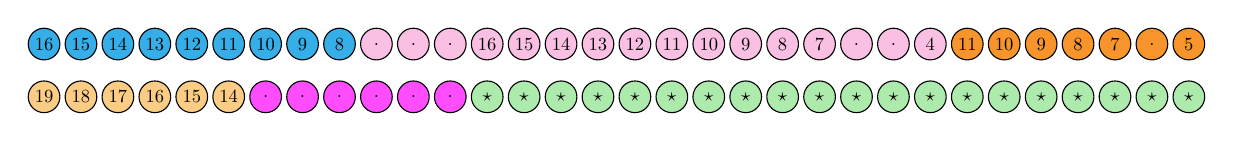
\begin{tikzpicture}[scale=0.67,transform shape]
\draw[fill=Cerulean!85] (0,0) circle (.3) node{16};
\draw[fill=Cerulean!85] (0.7,0) circle (.3) node{15};
\draw[fill=Cerulean!85] (1.4,0) circle (.3) node{14};
\draw[fill=Cerulean!85] (2.1,0) circle (.3) node{13};
\draw[fill=Cerulean!85] (2.8,0) circle (.3) node{12};
\draw[fill=Cerulean!85] (3.5,0) circle (.3) node{11};
\draw[fill=Cerulean!85] (4.2,0) circle (.3) node{10};
\draw[fill=Cerulean!85] (4.9,0) circle (.3) node{ 9};
\draw[fill=Cerulean!85] (5.6,0) circle (.3) node{ 8};
\draw[fill=Rhodamine!30] (6.3,0) circle (.3) node{.};
\draw[fill=Rhodamine!30] (7.0,0) circle (.3) node{.};
\draw[fill=Rhodamine!30] (7.7,0) circle (.3) node{.};
\draw[fill=Rhodamine!30] (8.4,0) circle (.3) node{16};
\draw[fill=Rhodamine!30] (9.1,0) circle (.3) node{15};
\draw[fill=Rhodamine!30] (9.8,0) circle (.3) node{14};
\draw[fill=Rhodamine!30] (10.5,0) circle (.3) node{13};
\draw[fill=Rhodamine!30] (11.2,0) circle (.3) node{12};
\draw[fill=Rhodamine!30] (11.9,0) circle (.3) node{11};
\draw[fill=Rhodamine!30] (12.6,0) circle (.3) node{10};
\draw[fill=Rhodamine!30] (13.3,0) circle (.3) node{ 9};
\draw[fill=Rhodamine!30] (14.0,0) circle (.3) node{ 8};
\draw[fill=Rhodamine!30] (14.7,0) circle (.3) node{ 7};
\draw[fill=Rhodamine!30] (15.4,0) circle (.3) node{.};
\draw[fill=Rhodamine!30] (16.1,0) circle (.3) node{.};
\draw[fill=Rhodamine!30] (16.8,0) circle (.3) node{ 4};
\draw[fill=BurntOrange!85] (17.5,0) circle (.3) node{11};
\draw[fill=BurntOrange!85] (18.2,0) circle (.3) node{10};
\draw[fill=BurntOrange!85] (18.9,0) circle (.3) node{ 9};
\draw[fill=BurntOrange!85] (19.6,0) circle (.3) node{ 8};
\draw[fill=BurntOrange!85] (20.3,0) circle (.3) node{ 7};
\draw[fill=BurntOrange!85] (21.0,0) circle (.3) node{.};
\draw[fill=BurntOrange!85] (21.7,0) circle (.3) node{ 5};
\draw[fill=YellowOrange!45] (0,-1) circle (.3) node{19};
\draw[fill=YellowOrange!45] (0.7,-1) circle (.3) node{18};
\draw[fill=YellowOrange!45] (1.4,-1) circle (.3) node{17};
\draw[fill=YellowOrange!45] (2.1,-1) circle (.3) node{16};
\draw[fill=YellowOrange!45] (2.8,-1) circle (.3) node{15};
\draw[fill=YellowOrange!45] (3.5,-1) circle (.3) node{14};
\draw[fill=Fuchsia!70] (4.2,-1) circle (.3) node{.};
\draw[fill=Fuchsia!70] (4.9,-1) circle (.3) node{.};
\draw[fill=Fuchsia!70] (5.6,-1) circle (.3) node{.};
\draw[fill=Fuchsia!70] (6.3,-1) circle (.3) node{.};
\draw[fill=Fuchsia!70] (7.0,-1) circle (.3) node{.};
\draw[fill=Fuchsia!70] (7.7,-1) circle (.3) node{.};
\draw[fill=LimeGreen!40] (8.4,-1) circle (.3) node{$\star$};
\draw[fill=LimeGreen!40] (9.1,-1) circle (.3) node{$\star$};
\draw[fill=LimeGreen!40] (9.8,-1) circle (.3) node{$\star$};
\draw[fill=LimeGreen!40] (10.5,-1) circle (.3) node{$\star$};
\draw[fill=LimeGreen!40] (11.2,-1) circle (.3) node{$\star$};
\draw[fill=LimeGreen!40] (11.9,-1) circle (.3) node{$\star$};
\draw[fill=LimeGreen!40] (12.6,-1) circle (.3) node{$\star$};
\draw[fill=LimeGreen!40] (13.3,-1) circle (.3) node{$\star$};
\draw[fill=LimeGreen!40] (14.0,-1) circle (.3) node{$\star$};
\draw[fill=LimeGreen!40] (14.7,-1) circle (.3) node{$\star$};
\draw[fill=LimeGreen!40] (15.4,-1) circle (.3) node{$\star$};
\draw[fill=LimeGreen!40] (16.1,-1) circle (.3) node{$\star$};
\draw[fill=LimeGreen!40] (16.8,-1) circle (.3) node{$\star$};
\draw[fill=LimeGreen!40] (17.5,-1) circle (.3) node{$\star$};
\draw[fill=LimeGreen!40] (18.2,-1) circle (.3) node{$\star$};
\draw[fill=LimeGreen!40] (18.9,-1) circle (.3) node{$\star$};
\draw[fill=LimeGreen!40] (19.6,-1) circle (.3) node{$\star$};
\draw[fill=LimeGreen!40] (20.3,-1) circle (.3) node{$\star$};
\draw[fill=LimeGreen!40] (21.0,-1) circle (.3) node{$\star$};
\draw[fill=LimeGreen!40] (21.7,-1) circle (.3) node{$\star$};
\end{tikzpicture}
\end{center}
\caption{The inter-snippet buffer for steps $\state_{18}$ to $\state_{20}$.
From top to bottom, left to right, bright cerulean (\protect\tikz{\protect\draw[fill=Cerulean!85] (0,0) circle (.15);})
refers to bits from $\expmess_{16}$; light rhodamine (\protect\tikz{\protect\draw[fill=Rhodamine!30] (0,0) circle (.15);})
refers to bits from $\expmess_{15}$ (with some additional padding); bright (burnt) orange (\protect\tikz{\protect\draw[fill=BurntOrange!85] (0,0) circle (.15);})
bits come from $\expmess_{14}$, while light (yellow) orange (\protect\tikz{\protect\draw[fill=YellowOrange!45] (0,0) circle (.15);})
means bits from $\expmess_{17}$. Finally, bright fuchsia (\protect\tikz{\protect\draw[fill=Fuchsia!70] (0,0) circle (.15);})
and light lime (\protect\tikz{\protect\draw[fill=LimeGreen!40] (0,0) circle (.15);}) refer to padding bits
and bits holding the index of a base solution respectively.}
\label{fig:nb_packing80_1}
\end{figure}

\begin{figure}[!htb]
\begin{center}
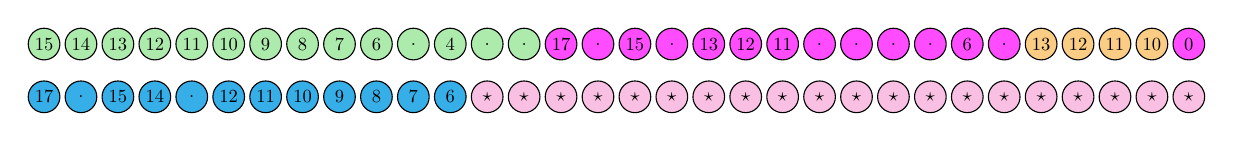
\begin{tikzpicture}[scale=0.67,transform shape]
\draw[fill=LimeGreen!40] (0,0) circle (.3) node{15};
\draw[fill=LimeGreen!40] (0.7,0) circle (.3) node{14};
\draw[fill=LimeGreen!40] (1.4,0) circle (.3) node{13};
\draw[fill=LimeGreen!40] (2.1,0) circle (.3) node{12};
\draw[fill=LimeGreen!40] (2.8,0) circle (.3) node{11};
\draw[fill=LimeGreen!40] (3.5,0) circle (.3) node{10};
\draw[fill=LimeGreen!40] (4.2,0) circle (.3) node{ 9};
\draw[fill=LimeGreen!40] (4.9,0) circle (.3) node{ 8};
\draw[fill=LimeGreen!40] (5.6,0) circle (.3) node{ 7};
\draw[fill=LimeGreen!40] (6.3,0) circle (.3) node{ 6};
\draw[fill=LimeGreen!40] (7.0,0) circle (.3) node{.};
\draw[fill=LimeGreen!40] (7.7,0) circle (.3) node{ 4};
\draw[fill=LimeGreen!40] (8.4,0) circle (.3) node{.};
\draw[fill=LimeGreen!40] (9.1,0) circle (.3) node{.};
\draw[fill=Fuchsia!70] (9.8,0) circle (.3) node{17};
\draw[fill=Fuchsia!70] (10.5,0) circle (.3) node{.};
\draw[fill=Fuchsia!70] (11.2,0) circle (.3) node{15};
\draw[fill=Fuchsia!70] (11.9,0) circle (.3) node{.};
\draw[fill=Fuchsia!70] (12.6,0) circle (.3) node{13};
\draw[fill=Fuchsia!70] (13.3,0) circle (.3) node{12};
\draw[fill=Fuchsia!70] (14.0,0) circle (.3) node{11};
\draw[fill=Fuchsia!70] (14.7,0) circle (.3) node{.};
\draw[fill=Fuchsia!70] (15.4,0) circle (.3) node{.};
\draw[fill=Fuchsia!70] (16.1,0) circle (.3) node{.};
\draw[fill=Fuchsia!70] (16.8,0) circle (.3) node{.};
\draw[fill=Fuchsia!70] (17.5,0) circle (.3) node{ 6};
\draw[fill=Fuchsia!70] (18.2,0) circle (.3) node{.};
\draw[fill=YellowOrange!45] (18.9,0) circle (.3) node{13};
\draw[fill=YellowOrange!45] (19.6,0) circle (.3) node{12};
\draw[fill=YellowOrange!45] (20.3,0) circle (.3) node{11};
\draw[fill=YellowOrange!45] (21.0,0) circle (.3) node{10};
\draw[fill=Fuchsia!70] (21.7,0) circle (.3) node{ 0};
\draw[fill=Cerulean!85] (0,-1) circle (.3) node{17};
\draw[fill=Cerulean!85] (0.7,-1) circle (.3) node{.};
\draw[fill=Cerulean!85] (1.4,-1) circle (.3) node{15};
\draw[fill=Cerulean!85] (2.1,-1) circle (.3) node{14};
\draw[fill=Cerulean!85] (2.8,-1) circle (.3) node{.};
\draw[fill=Cerulean!85] (3.5,-1) circle (.3) node{12};
\draw[fill=Cerulean!85] (4.2,-1) circle (.3) node{11};
\draw[fill=Cerulean!85] (4.9,-1) circle (.3) node{10};
\draw[fill=Cerulean!85] (5.6,-1) circle (.3) node{9};
\draw[fill=Cerulean!85] (6.3,-1) circle (.3) node{8};
\draw[fill=Cerulean!85] (7.0,-1) circle (.3) node{7};
\draw[fill=Cerulean!85] (7.7,-1) circle (.3) node{6};
\draw[fill=Rhodamine!30] (8.4,-1) circle (.3) node{$\star$};
\draw[fill=Rhodamine!30] (9.1,-1) circle (.3) node{$\star$};
\draw[fill=Rhodamine!30] (9.8,-1) circle (.3) node{$\star$};
\draw[fill=Rhodamine!30] (10.5,-1) circle (.3) node{$\star$};
\draw[fill=Rhodamine!30] (11.2,-1) circle (.3) node{$\star$};
\draw[fill=Rhodamine!30] (11.9,-1) circle (.3) node{$\star$};
\draw[fill=Rhodamine!30] (12.6,-1) circle (.3) node{$\star$};
\draw[fill=Rhodamine!30] (13.3,-1) circle (.3) node{$\star$};
\draw[fill=Rhodamine!30] (14.0,-1) circle (.3) node{$\star$};
\draw[fill=Rhodamine!30] (14.7,-1) circle (.3) node{$\star$};
\draw[fill=Rhodamine!30] (15.4,-1) circle (.3) node{$\star$};
\draw[fill=Rhodamine!30] (16.1,-1) circle (.3) node{$\star$};
\draw[fill=Rhodamine!30] (16.8,-1) circle (.3) node{$\star$};
\draw[fill=Rhodamine!30] (17.5,-1) circle (.3) node{$\star$};
\draw[fill=Rhodamine!30] (18.2,-1) circle (.3) node{$\star$};
\draw[fill=Rhodamine!30] (18.9,-1) circle (.3) node{$\star$};
\draw[fill=Rhodamine!30] (19.6,-1) circle (.3) node{$\star$};
\draw[fill=Rhodamine!30] (20.3,-1) circle (.3) node{$\star$};
\draw[fill=Rhodamine!30] (21.0,-1) circle (.3) node{$\star$};
\draw[fill=Rhodamine!30] (21.7,-1) circle (.3) node{$\star$};
\end{tikzpicture}
\end{center}
\caption{The inter-snippet buffer for steps $\state_{21}$ to $\state_{25}$.
From top to bottom, left to right, light lime bits (\protect\tikz{\protect\draw[fill=LimeGreen!40] (0,0) circle (.15);})
come from $\expmess_{18}$ (with a few trailing padding bits);
bright fuchsia (\protect\tikz{\protect\draw[fill=Fuchsia!70] (0,0) circle (.15);})
refers to bits from $\expmess_{20}$, including two ``flip'' bits on positions 17 and 0, and yellow-tinted orange bits (\protect\tikz{\protect\draw[fill=YellowOrange!45] (0,0) circle (.15);})
are from $\expmess_{17}$. Bright cerulean means (\protect\tikz{\protect\draw[fill=Cerulean!85] (0,0) circle (.15);})
bits from $\expmess_{19}$ (with two flip bits on 17 and 15), and finally light rhodamine (\protect\tikz{\protect\draw[fill=Rhodamine!30] (0,0) circle (.15);}) bits hold the index of an extended base solution.}
\label{fig:nb_packing80_2}
\end{figure}


\subsection{An example of colliding message pair}
\label{sec:colli_ex80}

We give an example of 80-step collision in \autoref{tbl:fscoll80}.
This shows the two (message, \iv) pairs with their (identical) resulting digest.
This table is formatted in the same way as the one of \autoref{sec:colli_ex76}.

\begin{table}[!htb]
\caption{A freestart collision for 80-step \shaone. Message and \iv bytes with differences are highlighted with \framebox{\color{LimeGreen}coloured boxes}.}\label{tbl:fscoll80}
\centering
\begin{tabular}{l l}
\toprule
 & Message 1\\
\midrule
\iv &  \hspace{-10mm}\texttt{ 50 6b 01 78 ff 6d 18 \framebox{\color{Cerulean}90 20} 22 91 fd 3a de 38 71 b2 c6 65 ea}\\
\midrule
$\mess$ & \texttt{ \framebox{\color{Cerulean}9d} 44 38 \framebox{\color{Cerulean}28 a5} ea 3d \framebox{\color{Cerulean}f0 86} ea a0 \framebox{\color{Cerulean}fa 77} 83 a7 \framebox{\color{Cerulean}36}}\\
      & \texttt{ \hspace{1.15mm}33\hspace{1.25mm} 24 48 \framebox{\color{Cerulean}4d af} 70 2a \framebox{\color{Cerulean}aa a3} da b6 \framebox{\color{Cerulean}79 d8} a6 9e \framebox{\color{Cerulean}2d}} \\
			& \texttt{ \framebox{\color{Cerulean}54} 38 20 \framebox{\color{Cerulean}ed a7} ff fb \framebox{\color{Cerulean}52 d3} ff 49 \framebox{\color{Cerulean}3f c3} ff 55 \framebox{\color{Cerulean}1e}} \\
			& \texttt{ \framebox{\color{Cerulean}fb} ff d9 \framebox{\color{Cerulean}7f 55} fe ee \framebox{\color{Cerulean}f2 08} 5a f3 \framebox{\color{Cerulean}12 08} 86 88 \framebox{\color{Cerulean}a9}} \\
\midrule
$\compress(\iv,\mess)$ & \hspace{-3.4mm} \texttt{ f0 20 48 6f 07 1b f1 10 53 54 7a 86} \\
& \texttt{f4 a7 15 3b 3c 95 0f 4b }\\
\bottomrule\\

\toprule
 & Message 2 \\
\midrule
$\diff\iv$ & \hspace{-10mm}\texttt{ 50 6b 01 78 ff 6d 18 \framebox{\color{RubineRed}91 a0} 22 91 fd 3a de 38 71 b2 c6 65 ea}\\
\midrule
$\diff\mess$ & \texttt{ \framebox{\color{RubineRed}3f} 44 38 \framebox{\color{RubineRed}38 81} ea 3d \framebox{\color{RubineRed}ec a0} ea a0 \framebox{\color{RubineRed}ee 51} 83 a7 \framebox{\color{RubineRed}2c}} \\
      & \texttt{ \hspace{1.15mm}33\hspace{1.25mm} 24 48 \framebox{\color{RubineRed}5d ab} 70 2a \framebox{\color{RubineRed}b6 6f} da b6 \framebox{\color{RubineRed}6d d4} a6 9e \framebox{\color{RubineRed}2f}} \\
			& \texttt{ \framebox{\color{RubineRed}94} 38 20 \framebox{\color{RubineRed}fd 13} ff fb \framebox{\color{RubineRed}4e ef} ff 49 \framebox{\color{RubineRed}3b 7f} ff 55 \framebox{\color{RubineRed}04}} \\
			& \texttt{ \framebox{\color{RubineRed}db} ff d9 \framebox{\color{RubineRed}6f 71} fe ee \framebox{\color{RubineRed}ee e4} 5a f3 \framebox{\color{RubineRed}06 04} 86 88 \framebox{\color{RubineRed}ab}} \\
\midrule
$\compress(\diff\iv,\diff\mess)$ & \hspace{-3.4mm} \texttt{ f0 20 48 6f 07 1b f1 10 53 54 7a 86}\\
& \texttt{f4 a7 15 3b 3c 95 0f 4b} \\
\bottomrule
\end{tabular}
\end{table}

\subsection{Complexity of the attack}
\label{sec:comp80}

To estimate the complexity of the attack, we may as in \autoref{sec:comp76} consider the production rate of partial solutions up to $\state_{60}$ and the corresponding probability of extending
these to a collision. However, the slower production rate (due to the higher number of conditions) would lead to a less reliable estimate than in the 76-step case. Thus, we choose instead to
consider partial solutions up to $\state_{40}$. On a good-performing \gtx, such solutions are produced at a rate of about 1030 per second. The probability that one of these results
in a collision is given by JLCA to be $2^{-35.58}$, leading to an expected time to collision of 577.16 days.
Recalling that one \gtx can compute $2^{31.8}$ \shaone compression functions per second, the complexity of the attack is thus of $2^{57.37}$ on such a GPU.
However, it should be noted that as for the 76-step attack, the average performance of the GPUs on an actual cluster slightly degrades compared to a single one. In our attack, we used
sixteen 4-GPU machines, which combined together led to an attack of complexity about $2^{57.5}$.
